\section{Camera Calibration in OpenCV}
Camera calibration is needed to obtain camera parameters like focal length and center point.
Further, it provides a method to correct distortions caused by the imperfect optics according to a certain distortion models.
For that, a set of images of a known pattern (usually a checkerboard) have to be taken from different view-points an angles.
These points provide the training data which is needed to estimate all the coefficients.

This section describes the theory behind the calibration process in OpenCV 4.3.0, which is the latest version at the time of writing this thesis.
\subsection{The pinhole camera model}
The functions OpenCV provides to calibrate the camera use the so-called pinhole camera model \cite{cv_calib}.
This model describes, how a 3D-point specified in world-coordinates ($P_w$) is transformed to a 3D-point in camera-coordinates ($P_c$) and then further projected onto the image plane ($p$). After this step, the point is described as a 2D-point in pixel coordinates.  Figure \ref{theory:pin} illustrates this setup.
\begin{figure}[ht]
	\centering
	%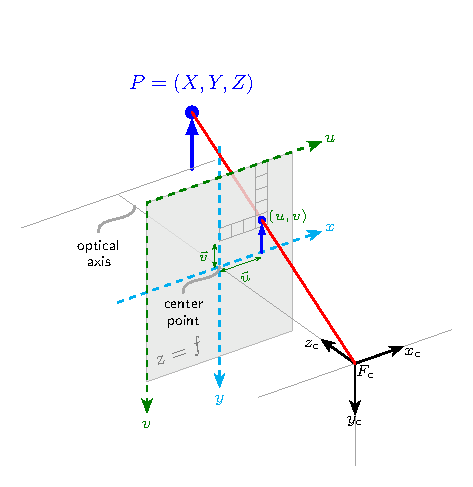
\includegraphics[width=0.9\textwidth]{2-theory/camera/camera.pdf}
	\caption{Pinhole-model (not up to date).\label{theory:pin}}
\end{figure} 

The transition from the world-coordinates to the camera-coordiantes can be described as 
\begin{align*}
\underbrace{\begin{pmatrix}
X_c\\
Y_c\\
Z_c\\
\end{pmatrix}}_{P_c}=
\underbrace{\begin{pmatrix}
r_{11}&r_{12}&r_{13}\\
r_{21}&r_{22}&r_{23}\\
r_{31}&r_{32}&r_{33}
\end{pmatrix}}_{R}
\underbrace{\begin{pmatrix}
X_w\\
Y_w\\
Z_w\\
\end{pmatrix}}_{P_w}+
\underbrace{\begin{pmatrix}
t_x\\
t_y\\
t_z\\
\end{pmatrix}}_{t}.
\end{align*}
The vector $P_w$ is first rotated by $R$ and the translated by $t$. This can be written in one single matrix:
\begin{align}
\begin{pmatrix}
X_c\\
Y_c\\
Z_c
\end{pmatrix}=
\begin{pmatrix}
r_{11}&r_{12}&r_{13}&t_x\\
r_{21}&r_{22}&r_{23}&t_y\\
r_{31}&r_{32}&r_{33}&t_z
\end{pmatrix}
\begin{pmatrix}
X_w\\
Y_w\\
Z_w\\
1
\end{pmatrix}\quad\Leftrightarrow\quad
P_c=
\begin{pmatrix}
R&|&t
\end{pmatrix}
\begin{pmatrix}
P_w\\
1
\end{pmatrix}\label{theory:world-camera}.
\end{align}

As a result of the theorem of intersecting lines, the projection from $P_c$ to $p$ is described as
\begin{align*}
\underbrace{\begin{pmatrix}
u\\
v
\end{pmatrix}}_{p}=
\begin{pmatrix}
f_x\cdot X_c/Z_c\\
f_y\cdot y_c/Z_c\\
\end{pmatrix}+
\begin{pmatrix}
c_x\\
c_y
\end{pmatrix}.
\end{align*}
where $f_x$ and $f_y$ are the focal length $f$ (in world units) normalized by their respective pixel size (in world units). Thus $f_x$ and $f_y$ are the same, if the pixels are quadratic.

By adding the principal point $\begin{pmatrix}c_x&c_y\end{pmatrix}^T$, which is usually close to the image center, it is taken into account, that pixel-coordinates are specified with respect to the upper left corner of the image plane. .
It is now simpler to write this in homogeneous coordinates:
\begin{align}
\begin{pmatrix}
u\\
v\\
1
\end{pmatrix}\sim s
\begin{pmatrix}
u\\
v\\
1
\end{pmatrix}=
\underbrace{\begin{pmatrix}
f_x&0&c_x\\
0&f_y&c_y\\
0&0&1
\end{pmatrix}}_{K}
\begin{pmatrix}
X_c\\
Y_c\\
Z_c
\end{pmatrix}\quad \Leftrightarrow \quad s
\begin{pmatrix}
p\\
1
\end{pmatrix}=
K\cdot P_c
\label{theory:camera-pixel},
\end{align}
where $s$ is an arbitrary scaling factor and $K$ is called the camera matrix.
The overall transition from world- to pixel-coordinates is the result of combining \ref{theory:world-camera} and \ref{theory:camera-pixel}:
\begin{align}
s
\begin{pmatrix}
u\\
v\\
1
\end{pmatrix}=
\begin{pmatrix}
f_x&0&c_x\\
0&f_y&c_y\\
0&0&1
\end{pmatrix}
\begin{pmatrix}
r_{11}&r_{12}&r_{13}&t_x\\
r_{21}&r_{22}&r_{23}&t_y\\
r_{31}&r_{32}&r_{33}&t_z
\end{pmatrix}
\begin{pmatrix}
X_w\\
Y_w\\
Z_w\\
1
\end{pmatrix}\quad \Leftrightarrow \quad s
\begin{pmatrix}
p\\
1
\end{pmatrix}=
K
\begin{pmatrix}
R&|&t
\end{pmatrix}
\begin{pmatrix}
P_w\\
1
\end{pmatrix}\label{theory:world-pixel}
\end{align}
The rotation and translation in $\begin{pmatrix}R&|&t\end{pmatrix}$ are called the extrinsic parameters. The camera matrix $K$ contains analogously the linear intrinsic parameters.

\subsection{The distortion model in OpenCV}
Non linear distortions, which appear before the projection in \ref{theory:camera-pixel} should be considered too.
OpenCV takes the effects of radial, tangential and thin prism distortion into account \cite{cv_calib}. 

\subsubsection{Radial Distortion}
Radial distortion is caused by the flawed curvature of the lens \cite{weng}.
It can be modeled with
\begin{align}
\begin{pmatrix}
x''\\
y''
\end{pmatrix}=
\begin{pmatrix}
x'\frac{1+k_1 r^2+k_2 r^4+k_3 r^6}{1+k_4 r^2+k_5r^4+k_6r^6}\\
y'\frac{1+k_1 r^2+k_2 r^4+k_3 r^6}{1+k_4 r^2+k_5r^4+k_6r^6}
\end{pmatrix}\label{theory:raddist},
\end{align}
where $x'$ and $y'$ are coordinates, described in camera-coordinates, normalized with $Z_c$
\begin{align*}
\begin{pmatrix}
x'\\
y'
\end{pmatrix}=
\begin{pmatrix}
X_c/Z_c\\
Y_c/Z_c
\end{pmatrix}
\end{align*}from
and r is the radius as taken with respect to the principal point $\begin{pmatrix}c_x&c_y\end{pmatrix}^T$
\begin{align*}
r^2 = x'^2 + y'^2.
\end{align*}
This type of distortion is symmetrical about the optical axis.
Figure \ref{theory:radial} illustrates the effect on a rectangle.
\begin{figure}[ht]
	\centering
	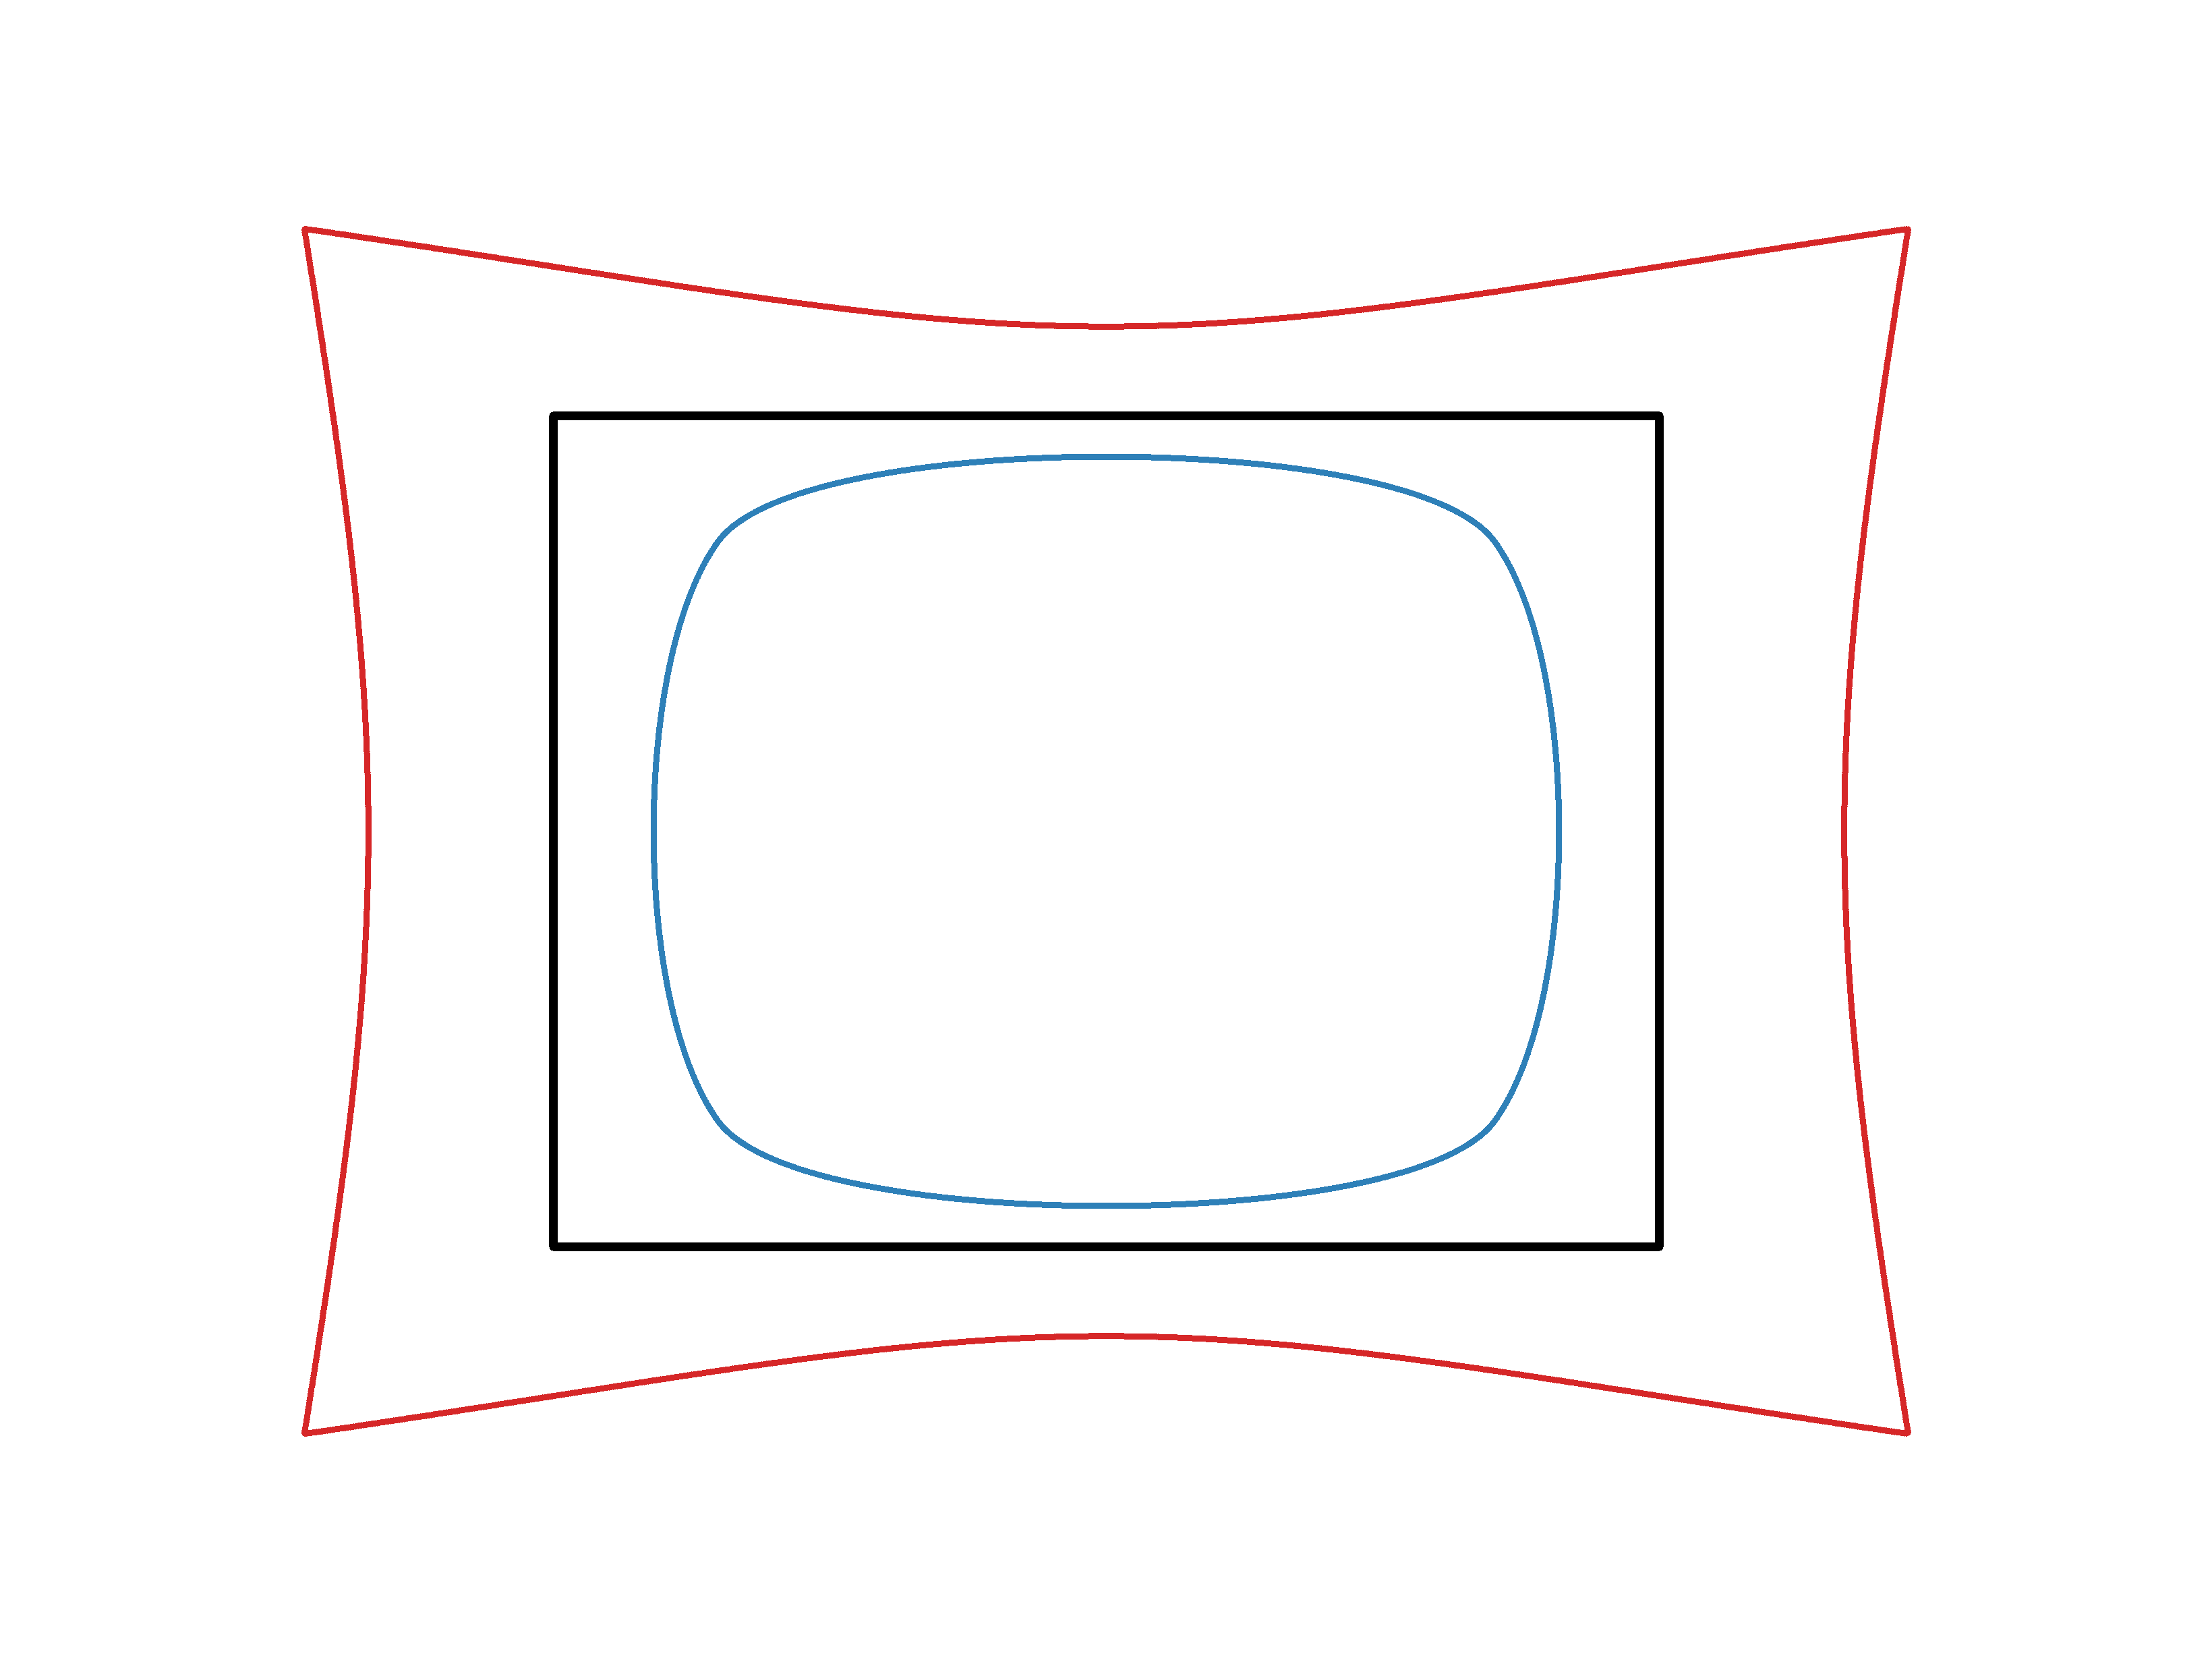
\includegraphics[width=0.9\textwidth]{2-theory/distortion/radial.png}
	\caption{Different types of radial distortion. Black: no distortion, red: $k_1 = 10$, $k_2=11$, $k_3=12$, $k_4=5$, $k_5=6$, $k_6=7$, blue: $k_1 = -2.2$, $k_2=-1.2$, $k_3=-0.8$, $k_4=-0.4$, $k_5=-0.3$, $k_6=-0.2$\label{theory:radial}}
\end{figure} 

\subsubsection{Tangential distortion}
Real optical systems are also subject to tangential distortion. This type of distortion has a decentering effect and occurs, if the line through the optical center of the lens and the principal point is not col-linear with the optical axis \cite{weng}.
The model
\begin{align}
\begin{pmatrix}
x''\\
y''
\end{pmatrix}=
\begin{pmatrix}
x' + 2p_1x'y'+p_2(r^2+2x'^2)\\
y' + 2p_2x'y'+p_1(r^2+2y'^2)
\end{pmatrix}\label{theory:tandist}
\end{align}
takes this into account.
Figure \ref{theory:tangential} shows the distortion this model introduces.

\begin{figure}[ht]
	\centering
	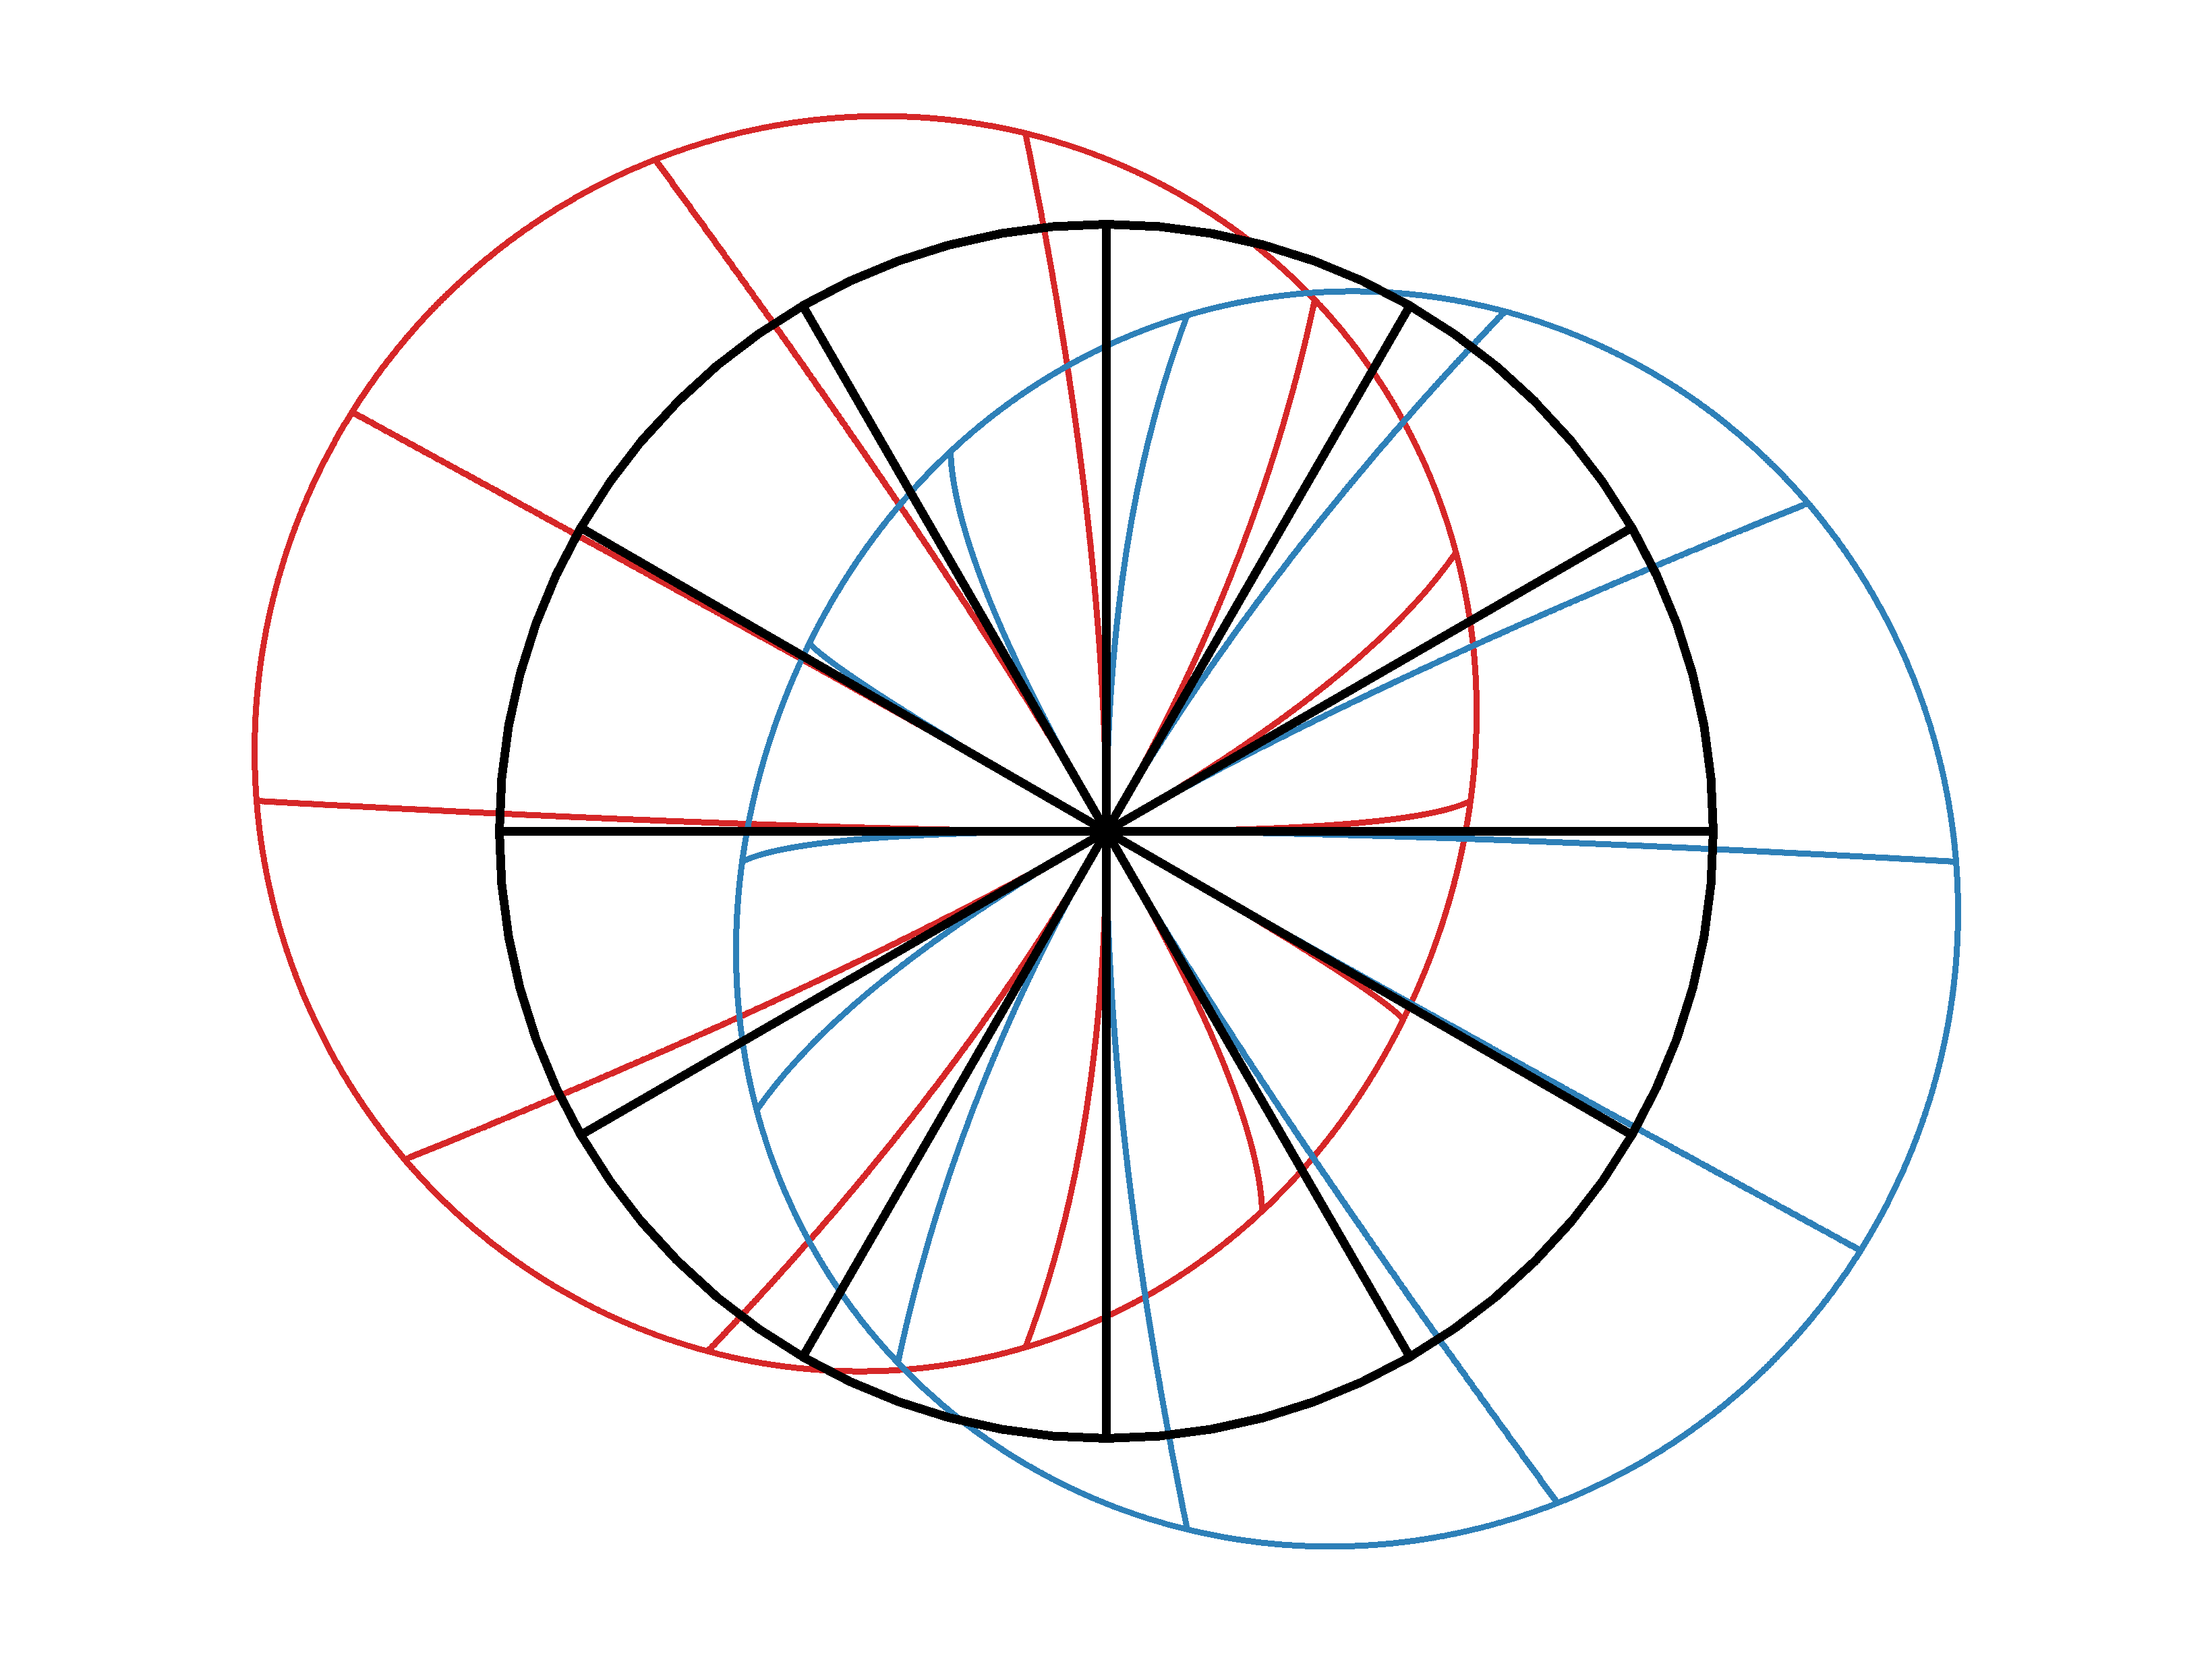
\includegraphics[width=0.9\textwidth]{2-theory/distortion/tangential.png}
	\caption{Different types of tangential distortion. Black: no distortion, red: $p_1 = -0.15$, $p_2=-0.4$, blue: $p_1 = 0.15$, $p2=-0.4$\label{theory:tangential}}
\end{figure} 

\subsubsection{Thin prism distortion}
Thin prism distortion is partially caused by lens imperfections and camera assembly \cite{weng}.
It introduces additional radial and tangential distortion, modeled with
\begin{align}
\begin{pmatrix}
x''\\
y''
\end{pmatrix}=
\begin{pmatrix}
x' + s_1 r^2 + s_2 r^4\\
y' + s_3 r^2 + s_4 r^4
\end{pmatrix}\label{theory:prismdist}.
\end{align}

\subsubsection{The combined model in OpenCV}
The models in \ref{theory:raddist}, \ref{theory:tandist} and \ref{theory:prismdist} combined result in
\begin{align}
\begin{pmatrix}
x''\\
y''
\end{pmatrix}=
\begin{pmatrix}
x'\frac{1+k_1 r^2+k_2 r^4+k_3 r^6}{1+k_4 r^2+k_5r^4+k_6r^6}+2p_1 x' y'+p_2(r^2+2x'^2)+s_1 r^2+s_2 r^4\\
y'\frac{1+k_1 r^2+k_2 r^4+k_3 r^6}{1+k_4 r^2+k_5r^4+k_6r^6}+2p_2x'y'+p_1(r^2+2y'^2)+s_3 r^2+s_4 r^4
\end{pmatrix}\label{theory:dist}.
\end{align}
In summary, a point in normalized camera-coordinates $\begin{pmatrix}x'&y'\end{pmatrix}^T$ is distorted as modeled in \ref{theory:dist}, which leads to the point $\begin{pmatrix}x''&y''\end{pmatrix}^T$. To get the distorted pixel-coordinates (subscript $d$), the projection has to be applied
\begin{align*}
\begin{pmatrix}
u_d\\
v_d\\
\end{pmatrix}=
\begin{pmatrix}
x''f_x+c_x\\
y''f_y+c_y
\end{pmatrix}\quad\Leftrightarrow\quad
\begin{pmatrix}
u_d\\
v_d\\
1
\end{pmatrix}=K
\begin{pmatrix}
x''\\
y''\\
1
\end{pmatrix},
\end{align*}
which completes the model so far.
Keep in mind, that when correcting the distortion, equation \ref{theory:dist} has to be inverted.

\subsection{Reprojection error}
The reprojection error is a value to asses the quality of a calibration.
It is the error between the detected image point and the projection (using the obtained coefficients) of its corresponding world point onto the image plane.
Since it only uses the points, which where previously used to obtain the calibration-parameters, it can be interpreted as a training error rate.

Calibration functions in OpenCV return the overall \acs{rms} reprojection error \cite{cv_calib}.

\subsection{Error propagation as further quality assessment}
As argued before, the reprojection error is a training error rate.
A low reprojection error is therefore not necessarily enough to estimate, how good the calibration really performs.

OpenCV returns with its extended calibration functions not only the camera intrinsics, but also an estimated standard deviation of each coefficient \cite{cv_calib}.
Under assumption that low standard deviations suggest a good calibration, it is valid to combine all standard deviations into one value using the propagation of uncertainty.

The propagation of error states that influence of each error of the inputs $x_i$ on the output value $y$ of a function
\begin{align*}
	y = f(x_1, x_2,..,x_n)
\end{align*}
can be linearly approximated and summed up to:
\begin{align}
	\Delta y = \sqrt{\sum_{i=1}^{n}\left(\frac{\partial y}{\partial x_i}\Delta x_i \right)^2} \label{theory:prop}.
\end{align}

Applied to \ref{theory:dist}, this leads to
\begin{align*}
	\Delta x''=\sqrt{\sum_{i=1}^{6}\left(\frac{\partial x''}{\partial k_i}\Delta k_i \right)^2+\sum_{i=1}^{2}\left( \frac{\partial x''}{\partial p_i}\Delta p_i\right)^2+\sum_{i=1}^{4}\left( \frac{\partial x''}{\partial s_i}\Delta s_i\right)^2}
\end{align*}
and
\begin{align*}
	\Delta y''=\sqrt{\sum_{i=1}^{6}\left(\frac{\partial y''}{\partial k_i}\Delta k_i \right)^2+\sum_{i=1}^{2}\left( \frac{\partial y''}{\partial p_i}\Delta p_i\right)^2+\sum_{i=1}^{4}\left( \frac{\partial y''}{\partial s_i}\Delta s_i\right)^2}.
\end{align*}
It is at this point not intended to go into further computations of the derivatives.
If we look at pixel coordinates from the center of the image, btw. $c_x=0$ and $c_y=0$, the radius (distance from the centerpoint) can be expressed as
\begin{align*}
	r = \sqrt{(f_x\cdot x'')^2+(f_y\cdot y'')^2}
\end{align*}
and therefore, if errors in $f_x$ and $f_y$ are neglected, with the propagation in \ref{theory:prop} applied
\begin{align}
	\Delta r = \sqrt{\left(\frac{\partial r}{\partial x''} \Delta x''\right)^2+\left(\frac{\partial r}{\partial y''} \Delta y''\right)^2}\label{theory:delta_r}.
\end{align}
This value $\Delta r$ can now be plotted over half the diagonal of an image to compare calibration coefficients of different calibration approaches.
